\section{Learning Outcomes}

By the end of week 3, you should be able to:

\begin{enumerate}
\item Understand the use of tab indents and colons.
\item Use {\tt if} statements.
\item Write {\tt while} and {\tt for} loops.
\item Use format strings (advanced).
\item Incorporate the {\tt range} function into your loops.
\item Use and define your own {\bf functions}.
\item Understand what {\tt lambda} functions are and when to use them (advanced).
\item Use the dictionary data type.

\end{enumerate}

\section{Colons and Indentation}

\label{indents}

\noindent Two important aspects of \texttt{Python} coding are indentation and colons, these help tell the program which parts of the code belong together when it comes to loops and if statements. These are not common to all programming languages (some use curly braces instead of indentation), but are vital for conditional statements, loops, and function definitions; three of the most important tools in programming.

\subsection*{Anatomy of Colons and Indentation}
\begin{figure}[H]  
\centering
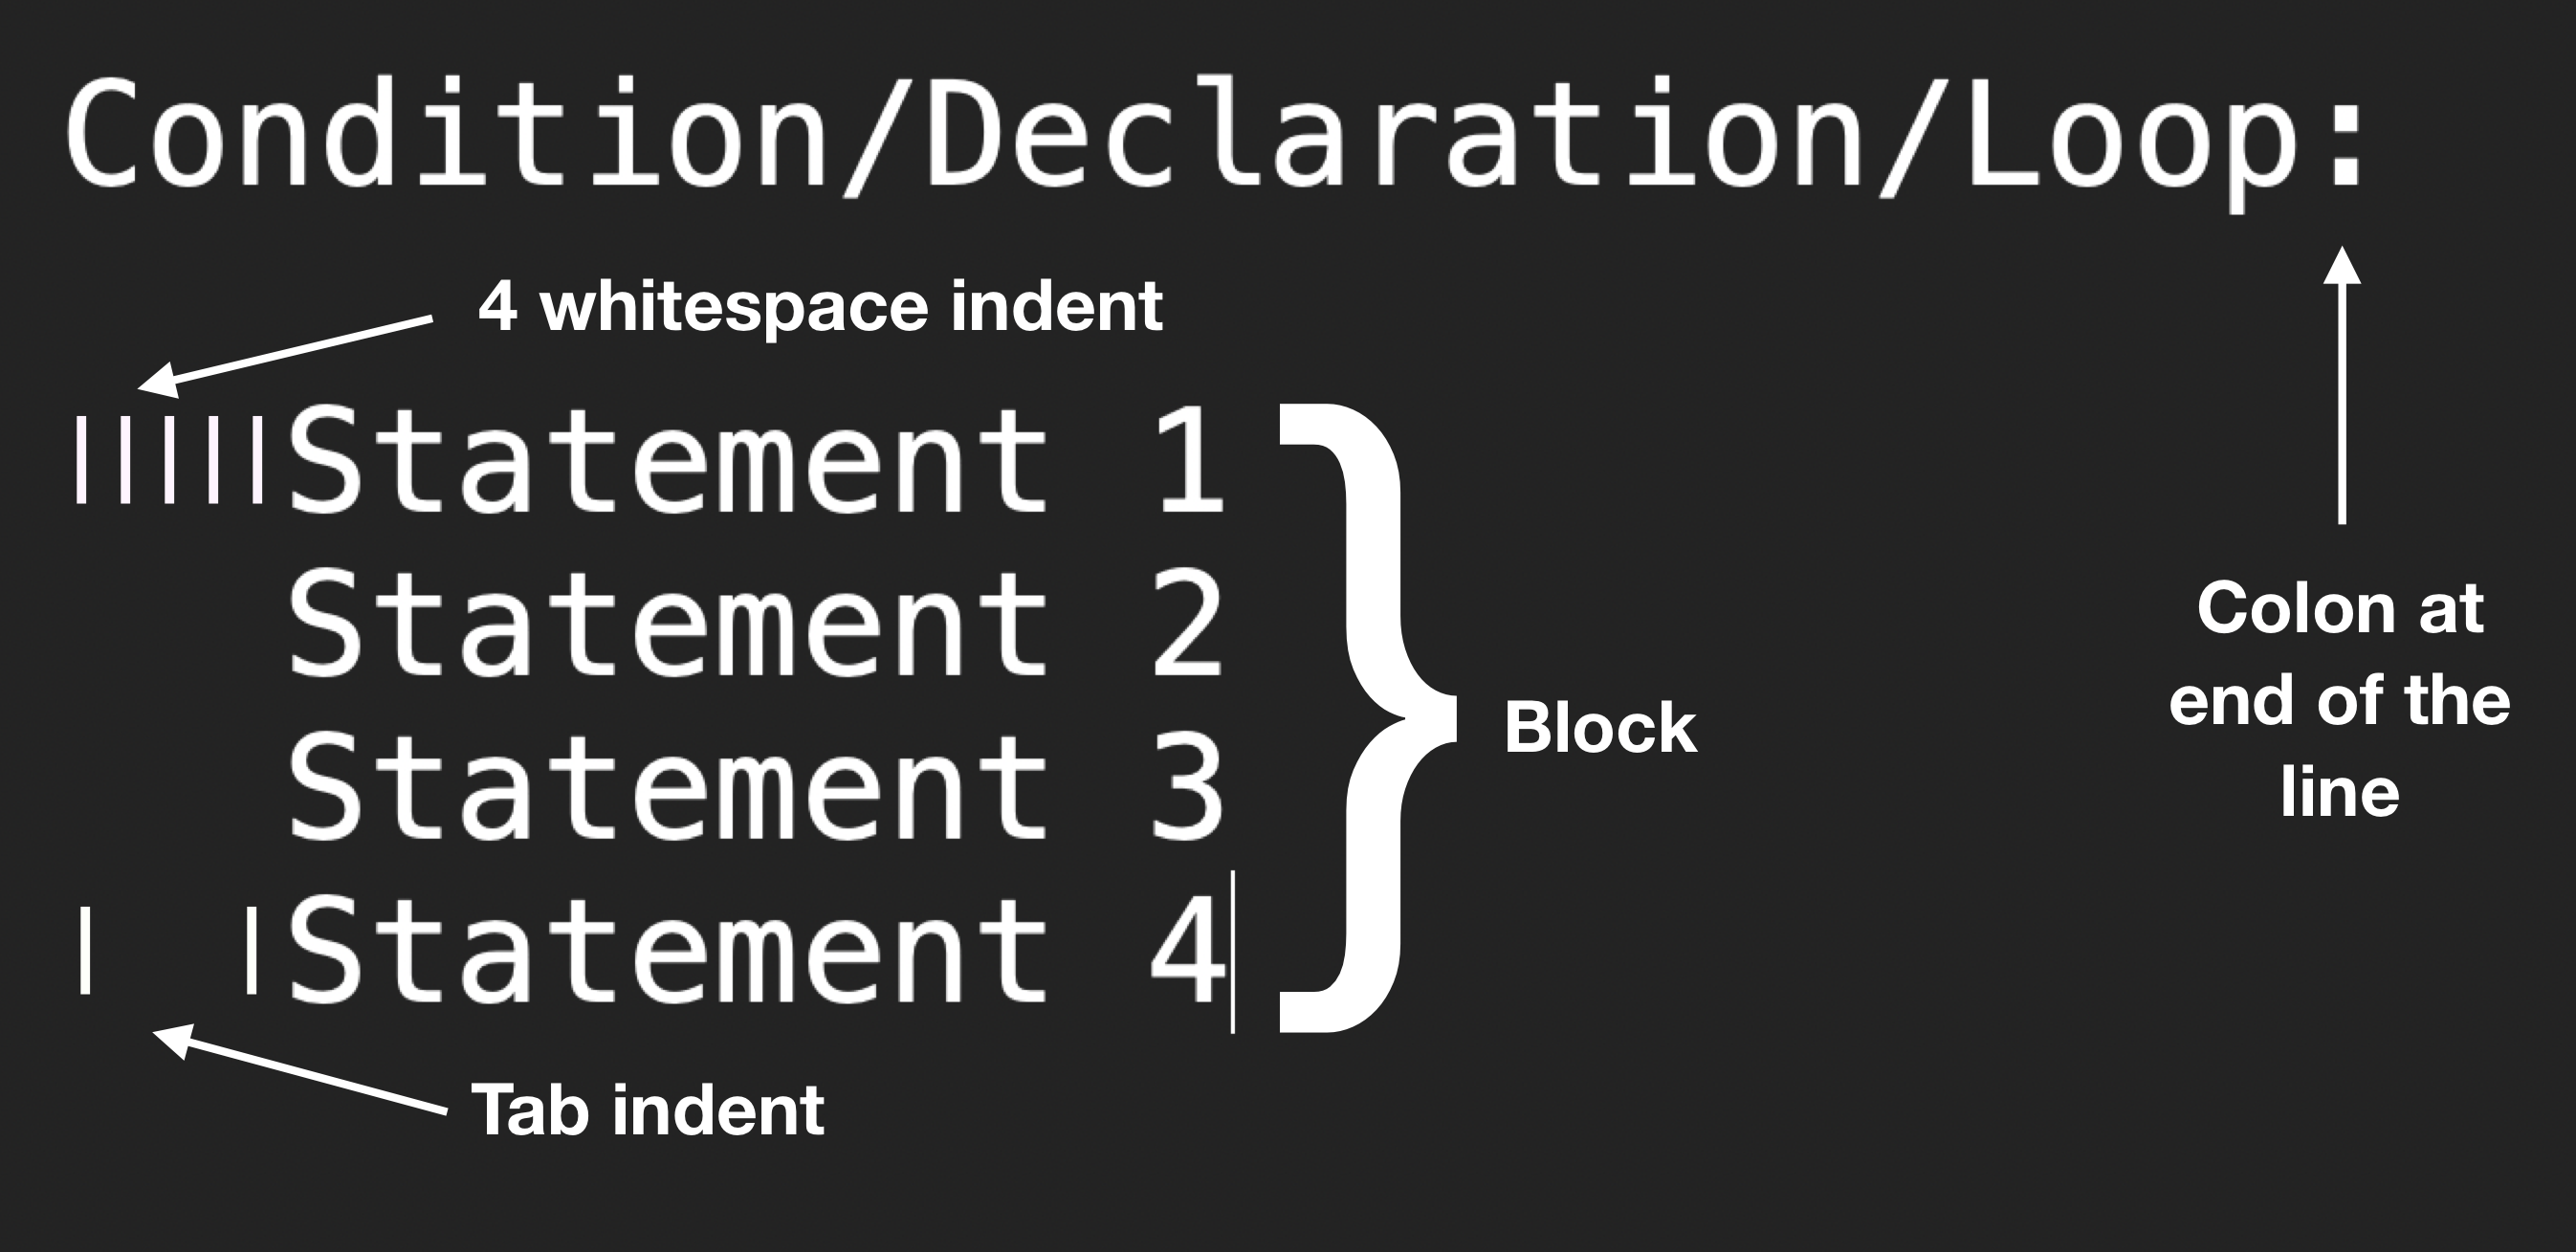
\includegraphics[width=0.7\linewidth]{Figures/anatomyOfColonindent.png}
\caption{A diagram showing the general form of a snippet of \texttt{Python} code using colons and indentation. Note: (as mentioned later) you can't mix whitespaces and tab indents, they are purely here for illustration.} 
\label{fig:colindt}
\end{figure}

\noindent {\bf Colons} are easy to forget, but are straight forward to use. You need to put one at the end of any \texttt{Python} command that is declaring a loop, condition (like an if statement), or function (as shown in Fig.\ref{fig:colindt}). If you forget to do that the code won't run and you'll be given a \texttt{SyntaxError} at the location of the line that is lacking one.
\vspace{0.1cm}

\noindent {\bf Indents} are similarly easy to forget, and you'll usually get an error message that tells you where you've forgotten to put one if you run the code. However, when things get a bit more complex and you have multiple nested loops and conditions it can be very easy to mis-indent a block or statement. This can be problematic, either introducing minor undesirable behaviours into your program, or a seriously detrimental bug. 

\noindent Time for an anecdote: One of the authors of this document managed to make 12TB of data overnight by accidentally indenting a single line of code one step further than it should have been. This caused the University of Sussex's high performance computing (HPC) cluster to fill up overnight, and induced mild panic in the department as everyone tried to clear unnecessary data out before important data was lost. So take this as cautionary tale: \textbf{Check your indents}.
\vspace{0.25cm}

\noindent An indent is, by convention, 4 "columns" ("white spaces") wide for \texttt{Python}, though it is possible to use one tab character instead - \textbf{using both in one script will not work}. In general Jupyter will add them for you if you've put a colon at the end of the previous line and then hit \keys{\enter}. If you need to put them in yourself, we recommend  using the tab key (although that does not work in all editors), rather than counting the number of times you've hit the space bar (which becomes extremely tedious).
\vspace{0.25cm}

\noindent Once a line, or series of lines, of code is indented, it is known as a \textbf{\textit{block}}. 

\noindent Learn to love indented code blocks: they are ubiquitous, powerful, and make the code more readable and easier to follow. Easily readable code is one of \texttt{Python's} main strengths and if you're ever handed a large program someone else has written you will truly begin to appreciate why this matters.

%\subsection{Exercises}

%ACTION - I need to find the code to run the slow counter
%W2Basic.7. Open the .ipynb file you used during the first lab session and find the cell where numbers from 1 to 5  are printed out slowly. See what happens if you remove the colon. See what happens if you remove each of the indents. See what happens if the indents are only, say, 2 spaces and not 4.


\section{The if statement}
The {\tt if} statement is a conditional construct. If a stated condition is met (is True), the code then executes a command or series of commands in the indented block following the colon. If statements are very useful and are used all the time in real codes.

\noindent The if statement allows a block of code run only if a condition is met. There are three types of if statements, \textbf{if}, \textbf{elif} and \textbf{else}. The `{\tt elif}' statement is short for `else if'  and allows for another conditional statement to be added to an existing if statement. If the `if' condition is not met, then the elif condition is tested, if this `{\tt elif}' condition is met then the `elif' block (statements indented below elif condition) is executed. If the condition of `{\tt elif}' is not true then that code block is also skipped.  The `{\tt else}' statement doesn't use an explicit condition (it has an implied condition simply meaning ``If none of the above was True"). For a visual interpretation of this see Fig.\ref{fig:iffc}.\\

\begin{figure}[h]
\vspace{-20pt}
\begin{center}
\resizebox{6.5cm}{!}{
\begin{tikzpicture}[node distance = 1cm, auto]
    \node [startend] (start) {};
    \node [question, below of=start, node distance=2cm] (ifcond) {\textbf{If condition}};
    \node [question, below of=ifcond, node distance=4cm] (elifcond) {\textbf{Elif condition}};
    \node [operation, below of=elifcond, node distance=4cm] (else) {\texttt{Else code}};
    \node [startend, below of=else, node distance=2cm] (end) {};
    \node [operation, right of=ifcond, node distance=7.5cm] (ifcode){\texttt{If code}};
    \node [operation, right of=elifcond, node distance=6.5cm] (elifcode){\texttt{Elif code}};
	\node [coord, below of=else, node distance=0.8cm](c1){};
	\node [coord, below of=else, node distance=1.3cm](c2){};

    \path [line] (start) -- (ifcond);
    \path [line] (ifcond) -- node {if condition True} (ifcode);
    \path [line] (ifcond) -- node {if condition False}(elifcond);
    \path [line] (elifcond) -- node{elif condition True}(elifcode);
    \path [line] (elifcond) -- node{elif condition False}(else);
    \path [line] (ifcode)|-(c2);
    \path [line] (elifcode)|-(c1);
    \path [line] (else) -- (end);
\end{tikzpicture}
}
\end{center}

\vspace{-20pt}
\caption{A generic ``if'' statement flow chart}
%\vspace{-10pt}
\label{fig:iffc}
\end{figure}

\noindent Note: you can have as many `{\tt elif}' statements in an `{\tt if}' construct as you like, but only one `{\tt else}' (this should make sense if you think about it). Neither statement is required though and each use case will define how the conditions should be approached. \\

\noindent Also note: unlike in some programming languages, in \texttt{Python} you do not need to spell out where the {\tt if} condition stops, i.e. there is no {\tt endif} statement. This is because the condition only applies to the indented lines of code.

% \noindent Below is an example of the combination of `if', `elif' and 'else' conditions and how they can be used.
% \begin{lstlisting}[style=PY]
% In [1]: if condition:
% 	        # indented code block 1
%         elif condition:
% 	        # indented code block 2
%         else:
% 	        # indented code block 3
% \end{lstlisting}

\noindent Here is a simple example of how to use an if statement (notice the structure of colons and indentation above (see Section~\ref{indents})): 
\begin{lstlisting}[style=PY]
In [2]: # Define a list of integers
        list1 = [0, 1, 2, 4, 5]
    
        # Test if the list contains 1 
        if 1 in list1:
            print('There is a one in list1')
        else:
            print('There is not a one in list1')
	    
\end{lstlisting}

\noindent Now run the cell, and you should receive the following output. 
\begin{lstlisting}[style=PY_out]
        There is a one in list1
\end{lstlisting}  
\noindent Now edit the cell and change \texttt{list1} to the following.
\begin{lstlisting}[style=PY]
        list1 = [0, 10, 2, 4, 5]
\end{lstlisting}
Running the code again then gives.
\begin{lstlisting}[style=PY_out]
        There is not a one in list1
\end{lstlisting}  
As you will see if you have done the task correctly, the `{\tt if}' condition was satisfied in the first case. In the second case it was not, hence the `{\tt else}' block was executed.\\

\noindent Here is another example, this time using an `{\tt elif}' statement (at this point you might want to revise Boolean statements from session 1). Note that this example introduces a way to do nothing in a code block, \texttt{\color{mygreen}pass}.
\begin{lstlisting}[style=PY, escapechar=\%] 
In [3]: # Define a variable containing an integer 
        a = 50
        
        # Test the value of the variable a
        if a == 50:
            print( 'Variable a is 50' )
        elif a > 100:
            print( 'Variable a is more than 100' )
        # Note that the next two lines do nothing, and can be omitted
        else:
            pass  # do nothing

        print ('Finished')
\end{lstlisting}

\noindent Running the code should produce the following result.
\begin{lstlisting}[style=PY_out]
        Variable a is 50
        Finished
\end{lstlisting}  
Now change {\it a} in the code to the following.
\begin{lstlisting}[style=PY]
        a = 120
\end{lstlisting}
\noindent Running it a second time should produce the following result.
\begin{lstlisting}[style=PY_out]
        Variable a is more than 100
        Finished
\end{lstlisting}  
\noindent As you can see the `{\tt elif}' condition was met and block executed.\\
\noindent Now change variable {\tt a} to the following.
\begin{lstlisting}[style=PY]
        a = 100
\end{lstlisting}
\noindent Now when running the code the following should appear.
\begin{lstlisting}[style=PY_out]
        Finished
\end{lstlisting}  
\noindent Now that the variable \texttt{a} is neither 50 or greater than 100, the `{\tt else}' condition is executed. In this case the code is simply \texttt{\color{mygreen}pass} which does nothing and continues with the remaining code. Pass is rarely advised(!) but if you were to leave this blank then an indentation error would occur. Try the example below and see what happens when you run it.
\begin{lstlisting}[style=PY, escapechar=\%]
In [4]: # Define a variable containing an integer 
        a = 10
        
        # Test the value of the variable a
        if a %\textbf{==}% 50:
            print('Variable a is 50')
        elif a > 100:
            print('Variable a is more than 100')

        print('Finished')
\end{lstlisting}
\noindent The example above should show you that you don't \textbf{have} to include `{\tt else}' statements with an `{\tt if}' statement, often there is no need for one. \\
You don't just have to use singular conditions for `{\tt if}' and `{\tt elif}' statements, you can combine conditions together using \texttt{and} \texttt{or} or any other Boolean combination, as in the following:
\begin{lstlisting}[style=PY]
In [5]: # Define a tuple of names 
        b = ("Neil", "Edwin", "Michael")
        
        # Test if certain names are within the tuple
        if "Edwin" or "Buzz" in b:
            print("Edwin 'Buzz' Aldrin was the second man on the moon.")
        # Note that the next two lines do nothing, and can be omitted
        else:
            pass
\end{lstlisting}
\noindent If the code above was run, the text would be printed if tuple {\tt b} contained `Edwin' or `Buzz'. The Boolean \textbf{\color{orange}not} operator could be used to reverse the output i.e True becomes False and vice-verse. For example the above code could be changed to:
\begin{lstlisting}[style=PY]
In [6]: # Define a tuple of names
    # Test if certain names are within the tuple
    if "Edwin" or "Buzz" not in b:
        print("One of his names is missing from the list!")
    # Note that the next two lines do nothing, and can be omitted
    else:
        None
\end{lstlisting}

\newpage
\begin{lstlisting}[style=PY]
In [7]: # Define a tuple of names
    b = ('Neil', 'Edwin', 'Michael')
    # Test if certain names are within the tuple
    if 'Neil' and 'Edwin' in b:
        print('Neil Armstrong and Edwin \'Buzz\' Aldrin were the first 
               men to set foot on the moon.')
    # Note that the next two lines do nothing, and can be omitted
    else:
        None
\end{lstlisting}
This time, the use of \textbf{\color{orange}and} prints the text since both conditions have been met. 
Here, we have used {\color{mygreen}\textbackslash'} to allow a quotation mark inside a string. The backslash tells \texttt{Python} to ignore parts of its own syntax and just use it as text within the string. Alternatively, you can define the string with double quotation marks to use a single quotation mark in the string, and vice versa. \\
\noindent Additionally you can combine (or ``nest'') `if' statements for example below:
\begin{lstlisting}[style=PY]
In [8]: # Define a list of numbers
        q = [2, 4, 6, 8]
        
        # Test the contents of the list with nested if statements
        if 2 in q:
            if 4 in q:
                if 6 in q:
                    if 8 in q:
                        print ('2, 4, 6 and 8 are in q')
                    else:
                        print ('2, 4 and 6 are in q')
                else:
                    print ('2 and 4 are in q')
            else:
                print ('2 is in q')
        # Note that the next two lines do nothing, and can be omitted
        else:
            pass
\end{lstlisting}
\noindent The indentations also help you see what is happening when using multiple \texttt{`if'} statements, (i.e. they make the code more `readable'), since each corresponding pair of \texttt{'if'} and \texttt{'else'} statements line up.

\subsection{Exercises}
\subsubsection{Exercises (with worked answers)}
\label{ifexercises}
\noindent Try the following examples. (The solutions can be found in section~\ref{workedanswerslab3}).
\begin{enumerate}
\item Create a list of names called \texttt{nlist}, then create a string variable called \texttt{myname}. Use an \texttt{if} statement to check if \texttt{myname} is not in \texttt{nlist}. If \texttt{myname} is not in the list, add the name to the list and print the list. If it is within the list, print the list. (At this point, you might need to revise the {\tt append} command from session 2.
\item
\begin{enumerate}
\item Set a variable called {\tt myscore} and assign an integer of between 0 and 100 to it. Then using {\tt  if} statements print (`You have a first') if {\tt myscore} is 70 or above, `You have a 2:1' if {\tt myscore} is between 60 and 69, `You have a 2:2' if {\tt myscore} is between 50 and 59, `You have a third' if {\tt myscore} is between 40 and 49 and  `You have a not passed' if {\tt myscore} is below 40.
\item Adapt your code so that if {\tt myscore} is above 100 or below 0, it replies that `{\tt myscore} is not within the correct boundaries'.
\item Adapt the code so that it asks for, and accepts, a value from the user. This value can be an integer or float.
\end{enumerate}
\end{enumerate}

\subsubsection{Exercises (other)}
\begin{enumerate}
    \item W3Basic1 - A leap year is defined as a year which is:
    \begin{itemize}
        \item Divisible by 4. \textbf{and}
        \item \textbf{Not} divisible by 100. \textbf{Unless} 
        \item It is divisible 400.
    \end{itemize}
    Using a single Jupyter cell, write a section of code that allows the user to input a year, then outputs `True' if the year is a leap year or `False' if it is not. [Hint: Make use of the modulo operator \%, if you have not come across modulo arithmetic the Wikipedia page is pretty good!]
    \item W3Basic2 - Write some \texttt{Python} commands in a Jupyter cell to check if an input number is positive, negative or zero.
\end{enumerate}

\section{While Loops}
When we want to perform a repetitive task in computing we call upon loops. Using loops incorrectly in your code can lead to ``infinite loops'', so please have a look at section \ref{sec:infiniloop} to remind yourself what to do if that happens.

There are two basic types of loop: {\tt while} loops and a {\tt for} loops. A while loop executes a piece of code while a condition is considered true.

\begin{figure}[h]
\begin{center}
\resizebox{0.4\linewidth}{!}{
\begin{tikzpicture}[node distance = 3cm, auto]
    \node [startend] (start) {};
    \node [question, below of=start, node distance=3cm] (while) {\textbf{While condition}};
    \node [coord, right of=while, node distance=4cm] (c1){};
    \node [operation, above of=c1, node distance = 1cm] (wcode) {\texttt{While code}};
    \node [startend, below of=while] (end) {};

    
    \path [line] (start) -- (while);
    \path [line] (while) -| node [below,text width =2.8cm]{while condition True} (wcode);
    \path [line] (wcode.north) |- (while.north);
    \path [line] (while) -- node {while condition False}(end);
\end{tikzpicture}
}
\end{center}
\caption{While loop flow chart}
\label{fig:wlfc}
\end{figure}
\vspace{1cm}
\noindent Until the `{\tt while}' condition is declared false, the code continues to execute the code block inside the \texttt{while} loop. In some cases a counter is used to make sure the condition will be declared false at some point (if it is never declared false, the code enters an infinite loop).  \\
\noindent In some cases an `{\tt else}' statement is used to invoke another code block, i.e. when the opposite of the {\tt while} condition is true. A basic flow chart in figure \ref{fig:wlfc} shows a while loop. Note the need for colons after the condition, and indented executable code (as was the case with the {\tt if} statement). \\

\noindent An example of a while loop can be seen below:
\begin{lstlisting}[style=PY]
In [1]: while condition:
            # code block 1
        else:
            # code block 2
\end{lstlisting}
Notice that you can also follow a while loop with an if statement. This essentially says "while the condition is true: execute the while block, once it is not true: execute the else block". \\


\noindent Try to work out what these while loops do and add appropriate comments:
\begin{lstlisting}[style=PY]
In [2]: x = 0
        while x <= 12:
            print(x)
            x = x + 1

        print('Done')
\end{lstlisting}
\noindent The example below contains an `if' statement nested in a while loop.
\begin{lstlisting}[style=PY]
In [3]: i = 1
        while i < 10:
            if i%2 == 0:
                print (i, ' is an even number')
            else:
                print (i, 'is an odd number')
            i = i + 1
\end{lstlisting}

\noindent In the example above \texttt{i = i +1} is used, this takes the variable \texttt{i} and adds one to it, an alternative syntax is:

\begin{lstlisting}[style=PY]
In [4]: i = 1
        i += 1
        i
\end{lstlisting}
\begin{lstlisting}[style=PY_out]
Out[4]: 2
\end{lstlisting}

\noindent The use of \texttt{i += n}, takes variable \texttt{i} and adds \texttt{n} to it and reassigns it to variable \texttt{i}. The examples below show how to similarly take a variable, and add, subtract, multiply or divide, then reassign the new value to that variable. These commands can be useful for counters.

 
\begin{lstlisting}[style=PY]
In [5]: i -= 1
        i
\end{lstlisting}
\begin{lstlisting}[style=PY_out]
Out[5]: 1
\end{lstlisting}
\begin{lstlisting}[style=PY]
In [6]: i *= 5
        i
\end{lstlisting}
\begin{lstlisting}[style=PY_out]
Out[6]: 5
\end{lstlisting}
\begin{lstlisting}[style=PY]
In [7]: i /= 2.0
        i
\end{lstlisting}
\begin{lstlisting}[style=PY_out]
Out[7]: 2.5
\end{lstlisting}


\subsection{Exercises}

\begin{enumerate}
    \item W3Basic3 - Write some code to do the following:
        \begin{enumerate}
            \item Ask a user to enter a start number, end number, and interval (i.e. step size).
            \item Then print out a series starting and ending at the defined values in steps of the desired interval.
        \end{enumerate}
\end{enumerate}

\newpage

\section{For Loops}
For loops are similar to while loops but they work through items in a sequence, executing a block of code each time. You will be using them a lot in this module.

\noindent {\it If you have not read the while loop section yet, please do so, as this section won't make sense otherwise!}

\vspace{1cm}
\begin{figure}[H]
\begin{center}
\resizebox{0.5\linewidth}{!}{
\begin{tikzpicture}[node distance = 3cm, auto]
    \node [startend] (start) {};
    \node [question, below of=start, node distance=3cm] (for) {\textbf{For item in sequence}};
    \node [coord, below of=for, node distance=2cm] (c1){};
    \node [operation,text width=6.2em, left of=c1, node distance = 3cm] (fcode) {\texttt{Executable code}};
    \node [startend, below of=for, right of=for] (end) {};

    
    \path [line] (start) -- (for);
    \path [line] (for) |- node [below,text width =2.8cm]{Next item in sequence} (fcode);
    \path [line] (fcode) |- (for);
    \path [line] (for) -| node [above,text width = 2.5cm]{No items left in sequence}(end);
\end{tikzpicture}
}
\end{center}
\caption{For loop flow chart}
\label{fig:flfc}
\end{figure}

\noindent One way to think of a for loop is that in the background a counter is active, performing a task until the counter reaches a certain number that is equal to the total items in a sequence. Just like \texttt{if} statements and while loops, for loops are written in the same way with a block, indented in to tell \texttt{Python} what to do.\\

\noindent Similar to \texttt{'while'} loops `else' statements can be used to perform an operation after the loop is complete. \texttt{'for'} loops can also be nested within each other to perform operations. An example layout of a for loop can be found below.

\begin{lstlisting}[style=PY]
In [1]: for item in sequence:
	        # code block 1
        else:
	        # code block 2
\end{lstlisting}
The sequence can be a range of numbers, a list, tuple, or even a string. The item is commonly referred to as `\texttt{i}' as it is a counter starting at the beginning of the sequence and stopping at the end, however we can name this counter variable anything within reason. (Because {\tt i} is so commonly used as a counter, \texttt{Python} uses {\tt j} to denote complex numbers, see session 1). \\

\newpage

\noindent This example prints out the result of a simple maths operation on a list of numbers.
\begin{lstlisting}[style=PY]
In [2]: # Define a list of numbers
        numberlist = [1, 2, 3, 4, 5, 6]
        
        # Loop over the elements in the list squaring them
        for i in numberlist:
            print (i*i)
\end{lstlisting}
This example prints each letter of a word on a new line. Here the sequence is a string, i.e. `{\tt word}'.

\begin{lstlisting}[style=PY]
In [3]: # Loop over the characters in a string printing each
        for letter in 'word':
            print (letter)
\end{lstlisting}
This example loops through a list of strings, printing the string and then it's length. Here the sequence is a list, i.e. `{\tt list1}'.
\begin{lstlisting}[style=PY]
In [4]: # Define a list of strings
        list1 = ['Monty', 'Python', 'Spam', 'Eggs']
        
        # Loop over the list printing the word and it's length
        for word in list1:
            print (word, 'has', len(word), 'letters')
\end{lstlisting}

\section{Format strings}
In the above example you will notice that when printing out the strings and integers or floats etc., parentheses and quotation marks are also printed. This is due to the fact we are mixing data types when printing, a way around this is to assign non-string types to variables and then use \emph{format strings} to print them.

A \emph{format string} is preceded by the letter f, and the variables to be
printed are enclosed in curly braces \{\}, e.g.
\begin{lstlisting}[style=PY]
  In [1]: # Example of format strings
  # Define a list of strings
        list1 = ['Monty', 'Python', 'Spam', 'Eggs']
        
        # Loop over the elements in the list 
        for word in list1:
        
            # Get word length
            wl = len(word)
            print(f'{word} has {wl} letters')
\end{lstlisting}

You can optionally specfify the format of the string conversion by following the variable name with a format qualifier, such as `:3d' to print a 3-digit integer, or `:5.4f' for a float with format x.xxxx.
\begin{lstlisting}[style=PY]
  In [1]: # Example of format strings with optional format specifier
  print(f'root 2 to 6 sig figs = {2**0.5:6.5f}')
\end{lstlisting}

%% The percentage symbol known as the {\bf modulo operator} in \texttt{Python}, allows for these data types to be inserted into a string, think of them as place holders. After the initial string there is a percentage symbol and a tuple or list containing the variables needed. Within the string itself you will see \texttt{\%s} the s converts the item in the tuple or list to a string for the print command, the order of the percentages in the string match the variables entered in the tuple or list, see example below. Some of the other commands are displayed in Table~\ref{tab:ms} they all allow variable values to be displayed in strings with different formatting.

%% \begin{lstlisting}[style=PY]
%% In [1]: # Define a list of strings
%%         list1 = ['Monty', 'Python', 'Spam', 'Eggs']
        
%%         # Loop over the elements in the list 
%%         for word in list1:
        
%%             # Get word length
%%             wl = len(word)
%%             print('%s has %s letters'%(word, wl))
%% \end{lstlisting}
%% %\begin{tcolorbox}[colback=red!5!white,colframe=red!75!black]
%% %\end{tcolorbox}
%% \begin{table}[H]
%% \begin{center}
%% \begin{tabular}{|l | p{12cm}|}
%% \hline
%% \texttt{\%s} & Converts variable to string.\\\hline
%% \texttt{\%i} & Converts variable to an integer in the string. To specifiy values use \texttt{\%ni} the n specifies how many characters are taken up for example if n was 5 and the variable was a 3 digit number two spaces would be in front of the variable or if n was 05 two zeros would be in front of the variable. If \texttt{\%i} is used the integer is just displayed.\\\hline
%% \texttt{\%d} & Converts variable to a decimal integer in the string. Similar to \texttt{\%i}\\\hline
%% \texttt{\%e} & Converts variable to an exponent in the form \texttt{w.nn e+xx} for use in string. If you wish to specify decimal places use the following \texttt{\%n.de}, the number would have d decimal places and the exponent n digits. E.g. \texttt{`\%2.3e'\% (45673)} would output \texttt{4.567e+04}.\\\hline
%% \texttt{\%f} & Converts variable to a float for use in string. To specify number of decimal places use \texttt{\%1.nf}, with n being number of decimal places e.g. \texttt{`\%1.2f'\% (25)} with output of \texttt{25.00}.\\\hline
%% \end{tabular}
%% \caption {String variable operators}
%% \label{tab:ms}
%% \end{center}
%% \end{table}

%% \begin{tcolorbox}[colback=red!5!white,colframe=red!75!black]
%% Although not needed for this sub-module, for completeness we note here that there is an alternative approach to the modulo command, the \texttt{.format} string function. It is much more powerful in usability, can have syntax uses and repetition of the same variable. and can inherently understand tuples. Additionally, as it is a function (Section~\ref{sec:function}), it can be used with map and other functions for more advanced \texttt{Python}. 

%% Again for completeness: if you're using \texttt{Python} $\geq$3.7 (the University isn't!) format strings have been introduced. These behave similarly to \texttt{.format} but are much more readable. To use a format string proceed your string by an f, i.e. \texttt{f''}.

%% \begin{lstlisting}[style=PY]
%% In [2]: # Define a list of numbers
%%         lst = [1.0, 9.9, 3.14159]
%%         approx_pi = lst[-1]
        
%%         # Using format
%%         print('The first element is {x}'.format(x=lst[0]))
%%         print('The last element is {x}'.format(x=approx_pi))
        
%%         # Using format strings (Python 3.7 or greater exclusive!)
%%         print(f'The first element is {lst[0]}')
%%         print(f'The last element is {approx_pi}')
%% \end{lstlisting}

%% \end{tcolorbox}

\newpage

\section{Range command}
\label{sec:range}
The \texttt{range} command allows you to create a list of numbers. You will be using it a lot in this module. Below are a few examples of the range command in action:
\begin{lstlisting}[style=PY]
In [1]: # Define a list using the range command containing 
        # integers from 0 to 9 (inclusive)
        list1 = range(10)
        print(*list1)
\end{lstlisting}
\begin{lstlisting}[style=PY_out]
        0 1 2 3 4 5 6 7 8 9
\end{lstlisting}

\noindent This is the range command in its simplest form, \texttt{range(j)}, it creates a list starting at zero with increments of 1 going all the way up to \texttt{j-1}. Note the \texttt{*}, this expands all the elements of a list (or tuple) rather than printing the list itself.

\begin{lstlisting}[style=PY]
In [2]: # Define a new list using range with a start and end point
        list2 = range(1, 11)
        print(*list2)
\end{lstlisting}
\begin{lstlisting}[style=PY_out]
        1 2 3 4 5 6 7 8 9 10
\end{lstlisting}
The above example shows the {\tt range} command with start and end declarations, i.e. the command \texttt{range(i,j)} creates a list starting at \texttt{i} and ending at \texttt{j-1} with increments of 1.
\begin{lstlisting}[style=PY]
In [3]: # Define a list using range with a start, end and step size
        list3 = range(0, 10, 2)
        print(*list3)
\end{lstlisting}
\begin{lstlisting}[style=PY_out]
        0 2 4 6 8
\end{lstlisting}
This final example shows the {\tt range} command with all of its inputs. \texttt{range(i,j,k)} where \texttt{i} is the start number, \texttt{j} declares the end (\texttt{j-1}) and \texttt{k} shows the step size. All of the inputs need to be integers as the range command only works with integers and not floats.\\
Table \ref{tab:rc} shows all the variants for the range command.
\begin{table}[H]
\begin{center}
\begin{tabular}{|l | p{7cm}|}
\hline
\multicolumn{2}{|c|}{\color{blue}Note: range command only works with integers}\\\hline
\texttt{range(j)} & Creates a list starting at 0 and ending at \texttt{j-1} with increments of 1\\\hline
\texttt{range(i,j)} & Creates a list starting at \texttt{i} and ending at \texttt{j-1} with increments of 1\\\hline
\texttt{range(i,j,k)} & Creates a list starting at \texttt{i} and ending at \texttt{j-1} with increments of \texttt{k}\\\hline
\end{tabular}
\end{center}
\caption {Range command}
\label{tab:rc}
\end{table}
\noindent Below is an example using the {\tt range} command and nested {\tt for} loops.
\begin{lstlisting}[style=PY]
In [4]: # Loop through a range 
        for i in range(2,6):
        
            print (f'{i} times table')
	        
            # Within the outer loop, loop over numbers between 1-10 
            for j in range(1,11):
	        
	        # Compute product of outer loop and inner loop integers
                num = i*j
		print (f'{i} x {j} = {num}')
\end{lstlisting}

\subsection{Using the separator command}

The separator command in {\tt print} is a nice feature.

\begin{lstlisting}[style=PY]
In [5]: # Define a list from a range 
        list4 = range(1, 11)
        
        # Print the list separated by whitespaces and commas
        print(*list4, sep=' , ')
\end{lstlisting}
\begin{lstlisting}[style=PY_out]
        1 , 2 , 3 , 4 , 5 , 6 , 7 , 8 , 9 , 10
\end{lstlisting}
The separator can indeed be anything, including ridiculous things.
\begin{lstlisting}[style=PY]
In [6]: print(*list4, sep='  [banana] ')
\end{lstlisting}
\begin{lstlisting}[style=PY_out]
        1 [banana] 2 [banana] 3 [banana] 4 [banana] 5 [banana] 6 [banana] 7 [banana] 8 [banana] 9 [banana] 10
\end{lstlisting}

\subsection{Exercises}
\subsubsection{Exercises (with worked answers)}
\label{rangeexercises}
\noindent Try the following examples. (The solutions can be found in section \ref{workedanswerslab3}).
\begin{enumerate}
\item Use a {\tt for} loop and the {\tt range} command to find the first 10 terms of the following series: $$\frac{1}{2}+\frac{1}{4}+\frac{1}{8}+\frac{1}{16}+\ldots$$
\item Using range, a for loop and if, elif and else conditions, print: \texttt{`1 potato 2 potato 3 potato 4, 5 potato 6 potato 7 potato more.'}.
\item Write an program that asks for and inputs the user's name. It then checks if the users name is within a list of names. If the name is in the list, it should then print a message telling the user that their name is on the list. If not, add the users name to the list and inform them their name has been added to the list.
\end{enumerate}

\subsubsection{Exercises (other)}

W3Basic4 - Write a program using a for loop that allows the user to input a word then print out the word backwards.
 
\section{Functions}
\label{sec:function}
There are already functions built into \texttt{Python}, {\tt print} for instance. However, you can also define your own functions. Functions are repeatable blocks of code that can be used over and over again. \\

\noindent Functions are defined using colons and indentation, similar to \texttt{if} statements and for/while loops. You can define parameters (arguments) to be used within the function, a general example is below:
\begin{lstlisting}[style=PY]
In [1]: def function_name( parameter1, parameter2,....):
            # block of code
            return statement(s)
\end{lstlisting}
Then to call upon them in the script use the following command.
\begin{lstlisting}[style=PY]
In [2]: function_name(x_parameter1, x_parameter2, ...)
\end{lstlisting}
Arguments don't have to be used, however they are used when performing tasks on different data points etc. An example not containing arguments is below:
\begin{lstlisting}[style=PY]
In [3]: def GameOver():
            print ('Game Over!')
            return

        GameOver()
\end{lstlisting}
Running the above code, will simply print out \texttt{Game Over!} when called upon, this simple example shows how repeatable code can save time as you don't have to write out the print command over and over again.

{\bf Be careful not to call your new function something that is already built in to \texttt{Python}!} You can check whether a function name is already in use by typing {\tt help(NameToCheck)}. As your coding gets more advanced, you will feel the benefits of using functions more and more. \\

\noindent The following example uses arguments:
\begin{lstlisting}[style=PY]
In [4]: def cubed(alist):

            # Loop over elements of the argument
            for i in range(len(alist)):
            
                # Cube the element and reassign it to the list
                alist[i] = alist[i]**3
                
        # Define a list of numbers to be used in the function
        numbers = list(range(5))
        
        # Cube the numbers using the user defined function
        cubed(numbers)
        print(numbers)
\end{lstlisting}

\noindent Running the code would output, \texttt{[0, 1, 8, 27, 64]}. Here, we have passed in the \texttt{numbers} variable, which was then assigned to a variable called \texttt{alist} in the function which is entirely internal to the function. 

\begin{lstlisting}[style=PY]
In [5]: def series(para):

            # Define a variable to hold the sum
            asum = 0
            
            # Loop over elements of the argument
            for i in para:
            
                # Sum the squares of the argument
                asum += para[i]**2
                
        # Define a list of numbers to be used in the function
        numbers = list(range(5))
        # Find the sum of the series defined by the function
        series(numbers)
        print(asum)
        
\end{lstlisting}
This code finds the sum of the series $x^{2}$, however if you have copied the code and run it yourself, you will find a NameError has occurred. This is due to \texttt{asum} not being a global variable i.e. it is only a variable within the function. To use this variable in different parts of the code we will need to return it, which will pass it back out of the function and assign it to another variable (this is part of a greater concept in coding called `Namespaces' [scopes in other languages] which will be covered later if people are interested).

\newpage

\begin{lstlisting}[style=PY]
In [6]: def series(para):

            # Define a variable to hold the sum
            asum = 0
            
            # Loop over elements of the argument
            for i in para:
            
                # Sum the squares of the argument
                asum += para[i]**2
                
            return asum
	    
        # Define a list of numbers to be used in the function
        numbers = list(range(5))
        
        # Find the sum of the series defined by the function
        series_sum = series(numbers)
        print (series_sum)
\end{lstlisting}

The return statement outputs the value, then we need to assign it to a variable, in this case \texttt{series\_sum}, to then read from it. If we wanted to return multiple values we can do the following:
\begin{lstlisting}[style=PY]
In [7]: def timestable(number):

            # Compute the products of the number in the argument
            a = number * 2
            b = number * 3
            c = number * 4
            d = number * 5
            
            return a, b, c, d
	        
        # Compute 5 multiplied by 2-5 (inclusive) using the function
        q, w, e, r = timestable(5) 
\end{lstlisting}
Using commas we can assign multiple variables with multiple returns. Side note here, a function returning multiple variables actually returns a tuple containing the returns.

\subsection{Exercises}
\begin{enumerate}
    \item W3Basic5 - Repeat W3Basic1 using a function.
    \item W3Basic6 - Repeat W3Basic2 using a function.
    \item W3Basic7 - Write a new function.
    \begin{enumerate} 
        \item It must take two parameters, a pay rate, and number of hours worked.
        \item Make it return the total pay.
        \item Alter the function so that any hours over 40 is paid at 1.5 times the normal rate.
    \end{enumerate}
\end{enumerate}

\section{Signpost} 

You need to have at least got to this point by the end of the lab session in week 3. You now have all the tools needed to finish the first assessment.

\begin{tcolorbox}[colback=red!5!white,colframe=red!75!black]
\section{Lambda statement}
The lambda statement is basically a single line function for use with expressions. The function can be expressed in the following way, with an arbitrary number of arguments:
\begin{lstlisting}[style=PY]
In [1]: function_name = lambda argument1, argument2, ...: expression
\end{lstlisting}
An example of a lambda statement:
\begin{lstlisting}[style=PY]
In [2]: root = lambda x, n: x**(1 / n)

        print (root(2,2))
        print (root(2,3))
        print (root(2,4))
\end{lstlisting}
Evidently, they are very similar to the function command but can be more succinct for simple repeatable calculations.
\end{tcolorbox}

\section{Dictionaries}
Although not used heavily in this course, dictionaries are one of the most powerful data structures in \texttt{Python}.

\noindent The dictionary data type holds pairs of {\bf keys} and {\bf values}, and are defined using curly braces `\{ \}'. The key, value pairs are defined as items with commas and a key separated by a `:'.\\

\noindent A dictionary cannot have any repeating keys, however it can have repeating values i.e. different keys can have the same value. An example of how to create a dictionary can be seen below, it also shows how to retrieve information from a particular key. Note that the values do not need to be strings, they can be numbers (e.g. phone numbers), or even \texttt{Python} objects.  
\begin{lstlisting}[style=PY]
In [1]: # Define a dictionary
        dictionary = {'key':'value', 'another key':'another value'}
        
        # Extract a value
        dictionary['key']
\end{lstlisting}
\begin{lstlisting}[style=PY_out]
Out[1]: 'value'
\end{lstlisting}
\begin{lstlisting}[style=PY]
In [2]: # Extract another value
        dictionary['another key']
\end{lstlisting}
\begin{lstlisting}[style=PY_out]
Out[2]: 'another value'
\end{lstlisting}

\newpage

\begin{lstlisting}[style=PY]
In [3]: # Define a dictionary with 2 of the same key
        double = {'key':1, 'key':2}
        double
\end{lstlisting}
\begin{lstlisting}[style=PY_out]
Out[3]: {'key': 2}
\end{lstlisting}
From the example above, you can see that if there is a repeating key the last value will be taken. Below are some more examples of manipulating dictionaries.
Here we reassign a string to an existing key overwriting the old value.
\begin{lstlisting}[style=PY]
In [1]: # Define a new dictionary
        dictionary = {'key':'old','Hello':'World'}
        
        # Overwrite the value of 'key'
        dictionary['key'] = 'new'
        dictionary['key']
\end{lstlisting}
\begin{lstlisting}[style=PY_out]
Out[1]: 'new'
\end{lstlisting}
We can delete a key using \texttt{Python}'s \texttt{del} function. This function deletes what follows it from memory (technically only removes the label/memory address) and is not specific to dictionaries. If you have a list that is hogging memory, but you no longer need it you can free up that memory using the \texttt{del} function (sort of: memory management is a somewhat mystic art in \texttt{Python}, ask if you are interested).
\begin{lstlisting}[style=PY]
In [2]: # Delete the entry under the key 'Hello'
        del dictionary['Hello']
        dictionary
\end{lstlisting}
\begin{lstlisting}[style=PY_out]
Out[5]: {'key':'new'}
\end{lstlisting}
You can add new keys:
\begin{lstlisting}[style=PY]
In [6]: # Assign a new entry to the dictionary
        dictionary['Good'] = 'bye'
        dictionary
\end{lstlisting}
\begin{lstlisting}[style=PY_out]
Out[6]: {'Good':'bye','key':'new'}
\end{lstlisting}
You can get the length of the dictionary which corresponds to the number of key, value pairs.
\begin{lstlisting}[style=PY]
In [7]: # Get the length of the dictionary
        len(dictionary)
\end{lstlisting}
\begin{lstlisting}[style=PY_out]
Out[7]: 2
\end{lstlisting}
You can also wipe a dictionary completely without deleting the data structure itself thusly:
\begin{lstlisting}[style=PY]
In [8]: # Wipe the contents of the dictionary
        dictionary.clear()
\end{lstlisting}
\begin{lstlisting}[style=PY_out]
Out[8]: {}
\end{lstlisting}

Below is a set of examples showing how you can access specific parts of a dictionary and interact with them.
We can get a list containing the items.
\begin{lstlisting}[style=PY]
In [9]: # Define 2 dictionaries for manipulation
        dict1 = {'Hello':'World','Good':'Bye'}
        dict2 = {'Game':'Over','You':'Lose'}
        
        # Get the items in a dictionary
        list(dict1.items())
\end{lstlisting}
\begin{lstlisting}[style=PY_out]
Out[9]: [('Hello','World'),('Good','Bye')]
\end{lstlisting}
We can get a list containing the keys.
\begin{lstlisting}[style=PY]
In [10]: # Get a list of the keys of a dictionary
         list(dict2.keys())
\end{lstlisting}
\begin{lstlisting}[style=PY_out]
Out[10]: ['Game','You']
\end{lstlisting}
We can get a list containing the values.
\begin{lstlisting}[style=PY]
In [11]: # Get a list of the values of a dictionary
         list(dict1.values())
\end{lstlisting}
\begin{lstlisting}[style=PY_out]
Out[11]]: ['World','Bye']
\end{lstlisting}
We can test if a key is within a dictionary.
\begin{lstlisting}[style=PY]
In [12]: # Test if 'Hello' is in the first dictionary
         if 'Hello' in dict1
\end{lstlisting}
\begin{lstlisting}[style=PY_out]
Out[12]: True
\end{lstlisting}
\begin{lstlisting}[style=PY]
In [13]: # Test if 'Hello' is in the second dictionary
         if 'Hello' in dict2
\end{lstlisting}
\begin{lstlisting}[style=PY_out]
Out[13]: False
\end{lstlisting}
We can combine dictionaries with the update method.
\begin{lstlisting}[style=PY]
In [14]: # Combine the 2 dictionaries
         dict1.update(dict2)
         dict1
\end{lstlisting}
\begin{lstlisting}[style=PY_out]
Out[14]: {'Hello':'World','Good':'Bye','Game':'Over','You':'Lose'}
\end{lstlisting}
The \texttt{dict.items()} function lists all the keys and values as tuples. The \texttt{dict.keys()} and \texttt{dict.values()} functions give the keys and values of the dictionary respectively. Finally the \texttt{dict.update()} adds the keys and values from one dictionary to another. - note that the ''()'' is important - the {\tt .key} etc. operations will not do anything without them. Think back to the function we defined with no arguments, the same would be true there. \\

\begin{tcolorbox}[colback=red!5!white,colframe=red!75!black]
\subsection{A Note On Iterators}
Here we have taken a small amount of poetic license. As of \texttt{Python} 3 a number of \texttt{Python}'s inbuilt functions were changed to return an object called an iterator rather than lists or tuples. This can greatly increase performance when simply looping through a set of keys, values or items in a dictionary but can also lead to some confusion when working with these. This is why all calls to \texttt{.items}, \texttt{.values} and \texttt{.keys} above are wrapped with \texttt{list()}.

You can work with the elements inside an iterator without issue when looping through them but should you find yourself needing to extract all values into a list and print them you would find that a \texttt{Python} object were printed instead. This is shown below

\begin{lstlisting}[style=PY]
In [1]: # Define a dictionary containing arbitrary keys and values
        dict1 = {'a': 1, 'b': 2, 'c': 3}
        print(dict1.keys())
        print(dict1.values())
        print(dict1.items())
\end{lstlisting}
\begin{lstlisting}[style=PY_out]
        dict_keys(['a', 'b', 'c'])
        dict_values([1, 2, 3])
        dict_items([('a', 1), ('b', 2), ('c', 3)])
\end{lstlisting}

To avoid this you can simply convert to a list or indeed a tuple as shown above depending on whether they need to be mutable or not.

\end{tcolorbox}

\section{Advanced Exercises}

Helpful hint: checking the glossary and the world wide web, may help with these exercises.

\begin{enumerate}

\item Write a program where a user gets 3 chances to guess a password. If the password is correct print `Access Granted' and exit the loop, if incorrect print `Access Denied'. Modify the code so that after the third guess a message is displayed telling the user they have run out of guesses.
\item DNA sequence strings are made up of the letters A, T, G, and C. The DNA sequence strings have a complement string where the the letters are switched. A's become T's,
T's become A's, G's become C's, and C's become G's. For example, the complement
of TTATGGCGTA is AATACCGCAT. Write a function that produces a complement of a DNA string.
\item Using a dictionary create a phone book, with a key of names and numbers as values. Then write a function that searches the dictionary for a name, if the name exists, give options to call, edit or remove the contact. If call is selected, print \texttt{Calling}, and the name, to the screen. Whereas, if edit of remove are selected, edit the number or remove the contact respectively. If the name does not appear give the option to add the name to the dictionary. 

\end{enumerate}

\newpage
\section{Worked Examples}
\label{workedanswerslab3}
\begin{lstlisting}[style=PY]
# 3.3.1
# Question 1.
myname = 'Nick' # Your name goes here  
nlist = ['Amy', 'Tom', 'Nina', 'James']
if myname not in nlist:
	nlist.append(myname)
	print (nlist)
else:
	print (nlist)
	
# Question 2a.
myscore = 65 # Your score would go here
if myscore > 70:
	print ('You have a first')
elif 60 <= myscore <= 69:
	print ('You have a two:one')
elif 50 <= myscore <= 59:
	print ('You have a two:two')
elif 40 <= myscore <= 45:
	print ('You have a third')
elif myscore < 40:
	print ('You have not passed')
	
# Question 2b.
myscore = 65 # Your score would go here
if 70 <= myscore <= 100:
	print ('You have a first')
elif 60 <= myscore <= 69:
	print ('You have a two:one')
elif 50 <= myscore <= 59:
	print ('You have a two:two')
elif 40 <= myscore <= 45:
	print ('You have a third')
elif 0 <= myscore <=40:
	print ('You have not passed')
else:
	print ('myscore is not within the boundary of 0 and 100')
\end{lstlisting}	
\newpage
\begin{lstlisting}[style=PY]
# Question 2c.
myscore = float(input('What is your score? '))
if 70 <= myscore <= 100:
	print ('You have a first')
elif 60 <= myscore <= 69:
	print ('You have a two:one')
elif 50 <= myscore <= 59:
	print ('You have a two:two')
elif 40 <= myscore <= 45:
	print ('You have a third')
elif 0 <= myscore <=40:
	print ('You have not passed')
else:
	print ('myscore is not within the boundary of 0 and 100')

3.6.2 
# Question 1
series = 0
for i in range (1,11):
	series += ( 1/(2.0**i) )
	print (series) 

# Question 2
string = ''
for num in range(1, 8):
    
    if num in [1, 2, 3, 5, 6]:
        string += str(num) + ' potato '
    elif num == 4:
        string += '4, '
    else:
        string += '7 potato more.'
        
print(string)

# Question 3.
names = ['Tom', 'Jerry', 'Sarah', 'Julian']
uname = input('Name? :')
if uname in names:
	print ('Your name is on the list')
else:
	name.append(uname)
	print ('Your name has been added to the list')
\end{lstlisting}
